% Credits are indicated where needed. The general idea is based on a template by Vel (vel@LaTeXTemplates.com) and Frits Wenneker.

\documentclass[11pt, a4paper]{article} % General settings in the beginning (defines the document class of your paper)
% 11pt = is the font size
% A4 is the paper size
% “article” is your document class

\input{general.tex} % Loads required packages from the separate file 

%---------------------------------------------------------------------------------
%	General information
%---------------------------------------------------------------------------------
\title{
\begin{figure}[h] % Defines figure environment
    \centering % Centers your figure
\includegraphics[scale=0.1]{figure/usblogo.png} % Includes your figure and defines the size
   % \caption{A circle} % For your caption
   % \label{fig:my_label} % If you want to label your figure for in-text references
\end{figure}
} % Adds your title
\author{
%FIRSTNAME LASTNAME % Add your first and last name
    %\thanks{} % Adds a footnote to your title
     \textit{www.stabolut.com} % Adds your institution
  }
\date{Version 0.7.4, \today} % Adds the version and the current date to your “cover” page

%---------------------------------------------------------------------------------
%	Define what’s in your document
%---------------------------------------------------------------------------------
\begin{document}
\maketitle % Print your title, author name and date;

\begin{abstract}
Stabolut is pioneering a dual-stablecoin strategy to address the diverse needs of the global digital economy. Our ecosystem features two distinct stablecoins: ESB, a Euro-pegged, MiCA-compliant Asset-Referenced Token (ART) for the European market, and USB, a US Dollar-pegged, decentralized stablecoin for international markets.

The entire Stabolut ecosystem is governed by the SBL token. SBL holders have the power to vote on key parameters for both ESB and USB, including risk management, treasury allocation, and the implementation of new features. This ensures that the Stabolut protocol remains a community-driven and decentralized project.

This whitepaper provides a comprehensive overview of the Stabolut ecosystem, detailing the architecture, mechanisms, and tokenomics of ESB, USB, and SBL.
\end{abstract}

\section*{Glossary}
\begin{description}
\item[ESB] Stabolut's MiCA-compliant, Euro-pegged stablecoin for the European market. It is an Asset-Referenced Token (ART) backed by a diversified portfolio of high-quality liquid assets and approved crypto-assets.

\item[USB] Stabolut's decentralized, US Dollar-pegged stablecoin for the international DeFi market. It is a yield-bearing token backed by a sophisticated crypto-hedging mechanism.

\item[SBL] Stabolut's utility and governance token. SBL holders can participate in governance decisions for both ESB and USB, and receive distributions from the Stabolut Treasury.

\item[Stabolut Treasury] A diversified pool of assets funded by the revenue generated from both ESB and USB. The treasury is used to fund the SBL buyback and burn program, as well as other ecosystem initiatives.

\item[Asset-Referenced Token (ART)] A type of stablecoin that is pegged to a basket of assets, including fiat currencies, commodities, and crypto-assets. ESB is an ART under MiCA regulations.

\item[Inverse Perpetual Swap] A type of derivative contract that allows Stabolut to hedge against the price volatility of crypto assets. This is the primary backing mechanism for USB.

\item[MiCA] The Markets in Crypto-Assets regulation, a comprehensive legal framework for crypto-assets in the European Union.
\end{description}

\input{content/toc} % Adds a table of content; 
%----------------------------------------------------------------------------------------
% Introduction
%----------------------------------------------------------------------------------------
\setcounter{page}{1} % Sets counter of page to 1
\section{Introduction}
Stabolut is pioneering a dual-stablecoin strategy to address the diverse needs of the global digital economy. Our ecosystem features two distinct stablecoins: ESB, a Euro-pegged, MiCA-compliant Asset-Referenced Token (ART) for the European market, and USB, a US Dollar-pegged, decentralized stablecoin for international markets.

\subsection{ESB: The MiCA-Compliant Euro Stablecoin}
ESB is designed to be a fully regulated and transparent stablecoin for the European Union. It is pegged to the Euro and backed by a reserve of high-quality liquid assets, in strict compliance with MiCA regulations. While ESB does not offer a direct yield, it provides value to users through a sophisticated system of transaction-based rewards, loyalty programs, and other MiCA-compliant incentives.

\subsection{USB: The Decentralized International Stablecoin}
USB is a decentralized, US Dollar-pegged stablecoin designed for the global DeFi market. It is backed by a basket of crypto assets and utilizes a sophisticated hedging mechanism to maintain its peg. USB is a yield-bearing token, offering a competitive return to holders in jurisdictions where such products are permitted.

\subsection{The SBL Governance Token}
The entire Stabolut ecosystem is governed by the SBL token. SBL holders have the power to vote on key parameters for both ESB and USB, including risk management, treasury allocation, and the implementation of new features. This ensures that the Stabolut protocol remains a community-driven and decentralized project.

This whitepaper provides a comprehensive overview of the Stabolut ecosystem, detailing the architecture, mechanisms, and tokenomics of ESB, USB, and SBL.
 % Adds your introduction
\section{A Dual-Stablecoin Strategy}
Stabolut employs a dual-stablecoin strategy to cater to the diverse regulatory landscapes and user needs of the global market. This approach allows us to offer a fully compliant, non-yield-bearing stablecoin for the European market, while also providing a decentralized, yield-bearing stablecoin for international users.

\begin{table}[h!]
\centering
\renewcommand{\arraystretch}{1.2}
\begin{tabular}{|l|p{6cm}|p{6cm}|}
\hline
\textbf{Feature} & \textbf{ESB (Euro Stablecoin)} & \textbf{USB (USD Stablecoin)} \\
\hline
\textbf{Target Market} & European Union & International / DeFi \\
\hline
\textbf{Peg} & Euro (EUR) & US Dollar (USD) \\
\hline
\textbf{Compliance} & MiCA-compliant ART & Decentralized \\
\hline
\textbf{Backing} & MiCA-compliant asset portfolio (including crypto-assets) & Crypto-asset hedging \\
\hline
\textbf{Yield} & No (reward-based) & Yes (yield-bearing) \\
\hline
\end{tabular}
\caption{ESB vs. USB: A Comparative Overview}
\label{tab:esbvsusb}
\end{table}

\subsection{ESB: The MiCA-Compliant Euro Stablecoin}
ESB is a fully regulated Asset-Referenced Token (ART) for the European market, pegged to the Euro. It is backed by a diversified and over-collateralized portfolio of MiCA-compliant assets, including approved crypto-assets such as Bitcoin and Ethereum.

\subsubsection{Compliant Crypto-Collateralization}
To be clear, ESB's reserve includes a carefully managed portfolio of crypto-assets, in full compliance with MiCA's requirements for Asset-Referenced Tokens. This is fundamentally different from the synthetic hedging mechanism used by USB.

The ESB reserve is a diversified portfolio of assets, including:
\begin{itemize}
    \item \textbf{High-Quality Liquid Assets}: A significant portion of the reserve is held in cash, bank deposits, and short-term government securities.
    \item \textbf{Approved Crypto-Assets}: A smaller portion of the reserve is held in a diversified basket of MiCA-compliant crypto-assets. Initially, this will be limited to Bitcoin (BTC) and Ethereum (ETH), selected for their unparalleled liquidity and market depth. The list of approved assets can be expanded by SBL governance, subject to regulatory approval.
\end{itemize}

The reserve is always over-collateralized to ensure that the value of the assets exceeds the value of the circulating ESB supply, even in the event of significant market volatility. This model provides the stability and security required by MiCA, while still allowing for a degree of exposure to the crypto markets.

\subsubsection{A Multi-Faceted Reward System for ESB}
ESB is designed to be an attractive and competitive stablecoin within the European market, despite not offering a direct yield. Its value proposition is built on a multi-faceted reward system that is fully compliant with MiCA regulations.

\begin{itemize}
    \item \textbf{Transactional Cashback}: Users receive a percentage of their transaction value back in ESB for every payment they make. The cashback rate is tiered based on monthly transaction volume, incentivizing high-frequency usage.
    \item \textbf{SBL Loyalty Program}: Users are rewarded with SBL tokens for their loyalty and engagement with the Stabolut ecosystem. SBL is earned by completing specific actions, such as:
    \begin{itemize}
        \item Onboarding new users to the platform.
        \item Participating in governance votes.
        \item Reaching specific milestones for the number of transactions.
    \end{itemize}
    \item \textbf{Fee Rebates}: High-volume users and merchants are eligible for significant rebates on transaction and service fees. This makes ESB a cost-effective solution for businesses and power users.
\end{itemize}

This activity-based reward structure ensures that ESB is not just a stable store of value, but also a dynamic and rewarding medium of exchange.

\subsubsection{Ensuring MiCA Compliance for ESB}
The ESB reward system is meticulously designed to comply with Article 40 of the MiCA regulation, which prohibits the granting of interest on e-money and asset-referenced tokens. The key to our compliance is the distinction between prohibited "interest" and permissible "activity-based rewards."

MiCA's prohibition targets remuneration that is linked to the duration of time a token is held. Our reward system, in contrast, is exclusively tied to user activity and engagement. As outlined in the provided regulatory analysis, this approach is fully compliant with MiCA's requirements.

The following table summarizes how our reward mechanisms align with MiCA's guidelines:

\begin{table}[h!]
\centering
\renewcommand{\arraystretch}{1.2}
\begin{tabular}{|l|p{6cm}|p{6cm}|}
\hline
\textbf{Reward Mechanism} & \textbf{How it Works} & \textbf{MiCA Compliance} \\
\hline
\textbf{Transactional Cashback} & Rewards are based on the volume and frequency of transactions. & Compliant, as the reward is triggered by payment activity, not passive holding. \\
\hline
\textbf{SBL Loyalty Program} & SBL tokens are earned by completing specific actions, such as referring new users or participating in governance. & Compliant, as the reward is based on user engagement and contribution to the ecosystem. \\
\hline
\textbf{Fee Rebates} & High-volume users receive discounts on transaction fees. & Compliant, as the benefit is directly linked to the user's activity level. \\
\hline
\end{tabular}
\caption{ESB Reward System: MiCA Compliance}
\label{tab:micacompliance}
\end{table}

By focusing on activity-based rewards, we ensure that ESB remains a compliant and attractive stablecoin for the European market, fostering a vibrant and engaged user base without violating MiCA's interest prohibition.

\subsection{USB: The Decentralized International Stablecoin}
USB is a decentralized, US Dollar-pegged stablecoin that is designed for the global DeFi market. It is backed by a sophisticated hedging mechanism that utilizes inverse perpetual swaps to maintain its peg to the US dollar.

\subsubsection{Yield Generation}
USB is a yield-bearing token that generates a competitive return for its holders. The yield is derived from the funding rates of the inverse perpetual swaps used in the hedging mechanism. This innovative approach allows USB to offer a stable and attractive yield, making it a compelling option for international users and DeFi protocols.

\textit{In our 2024 backtesting, the hedging strategy for ETH/USD funding rates generated an annualized yield of 60\%. When combined with the BTC/USD hedging strategy—which alone produced a yield of 16\% throughout 2024—this innovative approach significantly enhances the overall stability and income-generating profile of USB. It is important to note that past performance is not indicative of future results, and these figures should not be considered a guarantee of future returns.}

\section{Risk Management Framework}
Stabolut has implemented a comprehensive risk management framework to ensure the stability and security of the entire ecosystem. Our multi-layered approach to risk mitigation addresses the unique challenges of our dual-stablecoin model.

\subsection{Market Risk}
\begin{itemize}
    \item \textbf{ESB}: The ESB reserve is managed with a conservative asset allocation strategy. The crypto-asset portion of the reserve is over-collateralized and diversified across a basket of high-quality, liquid assets to mitigate price volatility.
    \item \textbf{USB}: The USB hedging mechanism is continuously monitored and adjusted to maintain a delta-neutral position. The Stabolut Treasury acts as a backstop to absorb any potential losses from extreme market events.
\end{itemize}

\subsection{Counterparty Risk}
\begin{itemize}
    \item \textbf{ESB}: All reserve assets are held by a diversified group of regulated and insured custodians, minimizing the risk of a single point of failure.
    \item \textbf{USB}: The hedging mechanism is distributed across a basket of reputable and liquid derivatives exchanges, reducing our exposure to any single counterparty.
\end{itemize}

\subsection{Regulatory Risk}
Our dual-stablecoin model is designed to be adaptable to the evolving global regulatory landscape. ESB is structured to be fully compliant with MiCA, while USB is offered in jurisdictions where yield-bearing stablecoins are permitted. This allows us to operate in a compliant manner across multiple regulatory regimes.

\subsection{Smart Contract Risk}
All smart contracts are subject to a rigorous, multi-phase audit process, including:
\begin{itemize}
    \item \textbf{Internal Audits}: Our in-house security team conducts a comprehensive review of all code before it is deployed.
    \item \textbf{Independent Audits}: We engage multiple, reputable third-party auditing firms to conduct independent reviews of our smart contracts.
    \item \textbf{Bug Bounties}: We offer a generous bug bounty program to incentivize the responsible disclosure of any vulnerabilities.
\end{itemize}

This multi-layered approach to security ensures that the Stabolut protocol remains a safe and reliable platform for our users.

\section{Transparency and Proof of Reserve}
Stabolut is committed to the highest standards of transparency and accountability. We believe that a robust and verifiable proof of reserve is essential for building trust and ensuring the long-term stability of our ecosystem.

\subsection{ESB: Audited Reserves}
The ESB reserve is subject to regular, independent audits by a reputable, third-party accounting firm. These audits will verify the composition and value of the reserve assets, ensuring that the ESB stablecoin is always fully backed by a diversified portfolio of MiCA-compliant assets. The audit reports will be made publicly available on a quarterly basis.

\subsection{USB: On-Chain Proof of Reserve}
For the USB stablecoin, we provide a real-time, on-chain proof of reserve. This is achieved through a publicly accessible dashboard that displays the following information:
\begin{itemize}
    \item The total value of the assets held in the hedging mechanism.
    \item The total number of USB tokens in circulation.
    \item The current collateralization ratio, which is always maintained above 100\%.
\end{itemize}

This on-chain transparency provides a continuous and verifiable proof of reserve, allowing users to monitor the health and stability of the USB stablecoin at any time.


 % Adds your Chapter 2
\section{SBL: The Unified Governance Token}
The SBL token is the cornerstone of the Stabolut ecosystem, providing a unified governance framework for both the ESB and USB stablecoins. SBL holders are empowered to make key decisions, ensuring that the protocol remains decentralized, transparent, and aligned with the interests of its community.

\subsection{The SBL Token Framework}
The SBL framework is built on five key pillars:
\begin{enumerate}
    \item \textbf{Unified Governance}: SBL holders have complete authority over the entire Stabolut ecosystem, including the ESB and USB stablecoins. This includes treasury allocations, fee structures, risk parameters, and protocol upgrades.
    \item \textbf{Treasury Surplus Distribution}: The Stabolut treasury is funded by the activities of both ESB and USB. SBL holders vote on the distribution of excess treasury funds, ensuring that the protocol's success is shared with the community.
    \item \textbf{Progressive Revenue Sharing}: A portion of the protocol's net revenue is distributed to SBL stakers, creating a direct link between protocol usage and token holder returns.
    \item \textbf{Deflationary Mechanisms}: The protocol can use treasury surplus to buy back and burn SBL tokens, reducing the circulating supply and increasing the value of the remaining tokens.
    \item \textbf{Utility Benefits}: SBL holders receive tangible benefits within the Stabolut ecosystem, such as reduced fees and enhanced voting power.
\end{enumerate}

\subsection{Progressive Staking and Governance}
To incentivize long-term commitment and active participation, Stabolut implements a progressive staking system with three tiers:

\begin{itemize}
    \item \textbf{Tier 1 (30-day lock)}: 1.2x voting multiplier, 5\% fee discount.
    \item \textbf{Tier 2 (180-day lock)}: 1.5x voting multiplier, 15\% fee discount.
    \item \textbf{Tier 3 (365-day lock)}: 2.0x voting multiplier, 30\% fee discount.
\end{itemize}

The rewards for progressive staking are calculated based on the user's staked SBL amount and their staking tier multiplier.

\begin{equation}
\text{User Reward} = (\frac{\text{User's Staked SBL} \times \text{Tier Multiplier}}{\sum (\text{All Staked SBL} \times \text{Tier Multipliers})}) \times \text{Total Reward Pool}
\end{equation}

This tiered system ensures that the most committed community members have the greatest influence on the protocol's direction and receive the most significant benefits.

\subsection{Treasury Surplus Distribution: A Democratic Approach to Value Creation}
The cornerstone of the SBL value accrual framework is the governance-controlled treasury surplus distribution mechanism. This mechanism is activated when the treasury's reserves exceed 25\% of the circulating stablecoin supply (both ESB and USB) plus a buffer for operational expenses.

When this threshold is met, SBL holders can vote on how to allocate the surplus funds. The available options are:

\begin{itemize}
    \item \textbf{Direct Airdrop}: A proportional distribution of the surplus funds to SBL holders.
    \item \textbf{Buyback and Burn}: The protocol uses the surplus to purchase SBL tokens on the open market and permanently removes them from circulation.
    \item \textbf{Yield Enhancement}: The surplus is deployed into additional yield-generating strategies, with the returns passed on to SBL stakers.
\end{itemize}

This democratic approach to value distribution ensures that the community has direct control over the protocol's economic engine, aligning the interests of the protocol with those of its token holders.

\subsection{Tokenomics: A Framework for Sustainable Growth}
The SBL tokenomics are meticulously designed to foster a sustainable and thriving ecosystem. The total supply is fixed at 1,000,000,000 SBL, ensuring scarcity and long-term value. The distribution model is strategically allocated to support the protocol's growth, reward early adopters, and incentivize community participation.

\subsubsection{SBL Token Distribution}
The allocation of SBL tokens is as follows:

\begin{table}[h!]
\centering
\renewcommand{\arraystretch}{1.2}
\begin{tabular}{|l|r|r|}
\hline
\textbf{Category} & \textbf{Allocation (\%)} & \textbf{No. of Tokens} \\
\hline
\textbf{Community Incentives} & \textbf{41.00\%} & \textbf{410,000,000} \\
\hline
Liquidity & 15.00\% & 150,000,000 \\
Ecosystem Reserve \& Growth & 10.00\% & 100,000,000 \\
Staking & 10.00\% & 100,000,000 \\
Airdrop & 7.00\% & 70,000,000 \\
Yield & 4.00\% & 40,000,000 \\
\hline
\textbf{Strategic Partners} & \textbf{15.00\%} & \textbf{150,000,000} \\
\hline
Core Team & 7.00\% & 70,000,000 \\
Strategic Advisors & 3.00\% & 30,000,000 \\
KOL & 5.00\% & 50,000,000 \\
\hline
\textbf{Fundraising} & \textbf{20.00\%} & \textbf{200,000,000} \\
\hline
Seed Round & 4.00\% & 40,000,000 \\
Private Round & 12.00\% & 120,000,000 \\
Public Round & 4.00\% & 40,000,000 \\
\hline
\textbf{Operational} & \textbf{24.00\%} & \textbf{240,000,000} \\
\hline
Reserve Funds & 12.00\% & 120,000,000 \\
Marketing & 7.00\% & 70,000,000 \\
\hline
\textbf{Total} & \textbf{100.00\%} & \textbf{1,000,000,000} \\
\hline
\end{tabular}
\caption{SBL Token Allocation}
\label{tab:tokenallocation}
\end{table}


\subsubsection{Vesting Schedule}
To ensure the long-term commitment of our strategic partners and team, a structured vesting schedule is in place. The number of vested tokens, $V(t)$, at a given time, $t$, is calculated as follows:

\begin{equation}
V(t) = 
\begin{cases} 
      0 & t < \text{cliff} \\
      \frac{T \times (t - \text{cliff})}{\text{vesting period}} & \text{cliff} \leq t \leq \text{vesting period} \\
      T & t > \text{vesting period}
   \end{cases}
\end{equation}

Where:
\begin{itemize}
    \item $T$ is the total number of tokens allocated to the individual or entity.
    \item $t$ is the time in months since the token generation event.
    \item The cliff is the initial period during which no tokens are vested.
    \item The vesting period is the total time over which the tokens are released.
\end{itemize}

This model ensures a gradual release of tokens, aligning the incentives of our partners with the long-term success of the protocol.


\subsubsection{Initial Valuation and Market Cap}
The initial valuation and market capitalization are as follows:
\begin{itemize}
    \item \textbf{Initial Circulating Supply}: 89,400,000 SBL
    \item \textbf{Initial Market Cap}: \$625,800
    \item \textbf{Fully Diluted Market Cap}: \$7,000,000
\end{itemize}

This structure provides a solid foundation for the SBL token, ensuring a balanced distribution that aligns the interests of all stakeholders and supports the long-term success of the Stabolut protocol.

\subsection{The SBL Value-Creation Cycle}
The SBL token is designed to appreciate in value through a self-reinforcing cycle fueled by the success of the entire Stabolut ecosystem. The Stabolut Treasury is the heart of this cycle, capturing value from both ESB and USB and distributing it to SBL holders.

\subsubsection{Treasury Revenue Streams}
The Stabolut Treasury is a single, unified entity that captures value from the entire ecosystem. It is funded by three primary revenue streams:
\begin{enumerate}
    \item \textbf{ESB Transaction Fees}: A small fee is charged on ESB transactions, which is directed to the treasury.
    \item \textbf{ESB Reserve Yield}: The yield generated from the high-quality liquid assets in the ESB reserve is another source of revenue for the treasury.
    \item \textbf{USB Yield Generation}: The yield generated from the inverse perpetual swaps used to back USB provides a consistent and substantial income stream from the international DeFi market.
\end{enumerate}

\subsubsection{The Value-Creation Flywheel}
The dual-revenue model creates a powerful flywheel effect for SBL value appreciation. This is achieved through a governance-controlled buyback and burn program, which is fueled by the Stabolut Treasury.

\begin{figure}[h!]
\centering
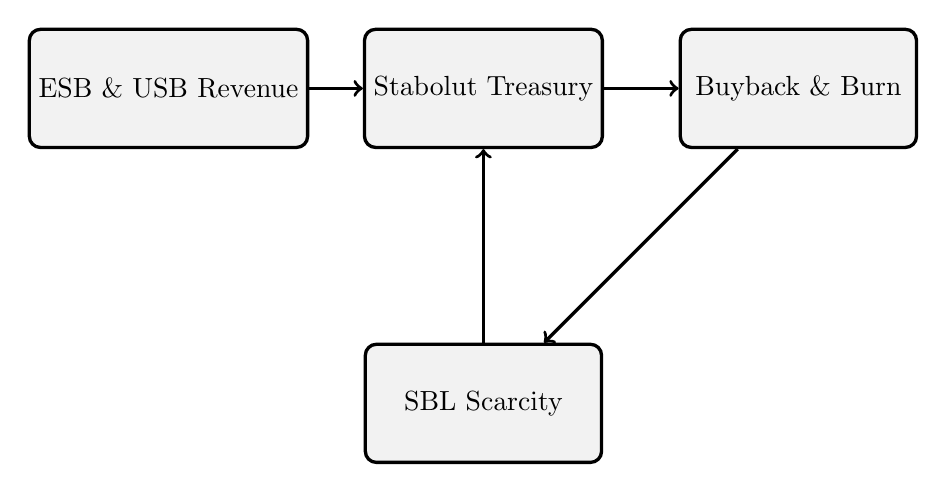
\begin{tikzpicture}
    [
        node/.style={rectangle, rounded corners, draw=black, fill=gray!10, very thick, minimum height=15mm, minimum width=30mm, text centered},
        arrow/.style={->, very thick}
    ]
    % Nodes
    \node[node] (revenue) at (0,0) {ESB \& USB Revenue};
    \node[node] (treasury) at (4,0) {Stabolut Treasury};
    \node[node] (buyback) at (8,0) {Buyback \& Burn};
    \node[node] (scarcity) at (4,-4) {SBL Scarcity};

    % Arrows
    \draw[arrow] (revenue) -- (treasury);
    \draw[arrow] (treasury) -- (buyback);
    \draw[arrow] (buyback) -- (scarcity);
    \draw[arrow] (scarcity) -- (treasury);
\end{tikzpicture}
\caption{The SBL Value-Creation Flywheel}
\label{fig:flywheel}
\end{figure}

\paragraph{The Buyback and Burn Mechanism}
The buyback and burn program is the primary driver of SBL value appreciation. When the Stabolut Treasury's reserves exceed 25\% of the total circulating stablecoin supply (ESB and USB), SBL holders can vote to allocate a portion of the surplus to the buyback and burn mechanism.

The amount to be used for the buyback, $B$, is calculated as follows:
\begin{equation}
B = (\text{Treasury Assets} - (0.25 \times \text{Circulating Stablecoin Supply})) \times \text{Burn Allocation \%}
\end{equation}


The number of SBL tokens to be burned, $SBL_{burned}$, is then determined by the current market price of SBL, $P_{SBL}$:
\begin{equation}
SBL_{burned} = \frac{B}{P_{SBL}}
\end{equation}

This process has a direct and immediate impact on the circulating supply of SBL, which in turn affects its market price. The new theoretical price of SBL, $P_{SBL'}$, can be modeled as:
\begin{equation}
P_{SBL'} = \frac{\text{SBL Market Cap}}{\text{Circulating Supply} - SBL_{burned}}
\end{equation}

This deflationary pressure, combined with the ongoing revenue generation from the ESB and USB ecosystems, creates a powerful and sustainable value accrual model for SBL holders.

The total value of the SBL token can be conceptualized as the sum of its base utility value, the net present value (NPV) of its future revenue share, the NPV of its future treasury surplus distributions, and a scarcity premium derived from the buyback and burn program.

\begin{equation}
\text{SBL Value} = \text{Base Utility} + \text{NPV(Revenue Share)} + \text{NPV(Surplus Distributions)} + \text{Scarcity Premium}
\end{equation}


\subsection{Regulatory Compliance and Investor Protection}

The SBL value accrual framework is designed to be fully compliant with the Markets in Crypto-Assets (MiCA) regulation. By structuring SBL as a utility token with governance rights and making distributions non-guaranteed and community-controlled, Stabolut mitigates the risk of SBL being classified as a security.

Key compliance features include:
\begin{itemize}
    \item \textbf{MiCA-Compliant Framework}: The SBL tokenomics are designed to align with MiCA's requirements for utility tokens.
    \item \textbf{Governance Control}: SBL holders have full control over the treasury surplus distribution, ensuring a decentralized and democratic process.
    \item \textbf{Legal Oversight}: All major governance decisions are subject to legal review to ensure ongoing compliance with MiCA and other global regulations.
\end{itemize}

 % Adds your Chapter 3 
\section{Use Cases}
The Stabolut ecosystem, with its dual-stablecoin model, is designed to serve a wide range of use cases across both traditional and decentralized finance.

\subsection{ESB: The MiCA-Compliant Euro Stablecoin}
ESB is the ideal stablecoin for the European market, offering a fully regulated and transparent solution for a variety of use cases:
\begin{itemize}
    \item \textbf{E-commerce and Point-of-Sale}: ESB provides a stable and efficient payment method for online and in-person transactions, with low fees and instant settlement.
    \item \textbf{Remittances and Cross-Border Payments}: ESB offers a cost-effective and compliant solution for sending and receiving money within the Eurozone.
    \item \textbf{Corporate Treasury Management}: ESB provides a stable and reliable asset for businesses to manage their cash reserves and make payments.
\end{itemize}

\subsection{USB: The Decentralized International Stablecoin}
USB is a versatile and yield-bearing stablecoin for the global DeFi market, with a wide range of use cases:
\begin{itemize}
    \item \textbf{Trading and Liquidity Provision}: USB is an ideal trading pair on decentralized exchanges, and its yield-bearing nature makes it an attractive asset for liquidity providers.
    \item \textbf{Lending and Borrowing}: USB can be used as collateral for loans or as a stable asset to lend out and earn a competitive yield.
    \item \textbf{Store of Value}: USB provides a stable and secure store of value for users in volatile markets, with the added benefit of a sustainable yield.
\end{itemize} 

 % Adds your Chapter 4
\section{Market Opportunity: A \$2.8 Trillion Addressable Market}

\subsection{The Dual Market Opportunity: Stablecoins and DeFi Governance Tokens}
The Stabolut protocol is uniquely positioned to capture value from two of the largest and fastest-growing sectors in the digital asset economy: stablecoins and DeFi governance tokens.

The stablecoin market, currently valued at over \$240 billion, is projected to grow to over \$2.8 trillion by 2028. This growth is driven by the increasing demand for a stable medium of exchange in the volatile cryptocurrency markets, as well as the growing adoption of stablecoins for cross-border payments, remittances, and decentralized finance (DeFi).

The market for DeFi governance tokens, while smaller, is also experiencing explosive growth. As the DeFi ecosystem matures, the need for robust and decentralized governance mechanisms is becoming increasingly critical. SBL, with its comprehensive value accrual framework and democratic control over the Stabolut protocol, is well-positioned to become a leading governance token in the DeFi space. The value of a governance token is derived from the right to vote on protocol parameters and to control the distribution of treasury funds.

\subsection{Target Markets and Use Cases}
Stabolut's dual-token architecture allows it to address a wide range of use cases and target markets:

\begin{itemize}
    \item \textbf{Cryptocurrency Exchanges}: USB provides a stable and reliable medium of exchange for traders, while SBL offers a compelling investment and governance opportunity.
    \item \textbf{DeFi Protocols}: USB can be integrated as a stable collateral asset in lending, borrowing, and derivatives protocols, while SBL can be used to govern these integrations.
    \item \textbf{Institutional Services}: The regulatory-compliant design of the Stabolut protocol makes it an attractive option for institutional investors and financial service providers.
    \item \textbf{Payment Providers}: The low transaction fees and fast settlement times of USB make it an ideal solution for cross-border payments and remittances.
\end{itemize}

By addressing these diverse markets, Stabolut is well-positioned to become a cornerstone of the digital asset economy.   % Adds your Chapter 5
\section{Roadmap}
Our roadmap is divided into two parallel tracks, one for the development of ESB and the other for the ongoing enhancement of USB.

\subsection{ESB: The MiCA-Compliant Euro Stablecoin}
\begin{itemize}
    \item \textbf{Q3 2025}: Finalize legal and regulatory framework for ESB and submit application for ART license under MiCA.
    \item \textbf{Q4 2025}: Launch private beta for ESB with a select group of institutional partners.
    \item \textbf{Q1 2026}: Launch public beta for ESB and begin integration with European payment providers.
    \item \textbf{Q2 2026}: Full public launch of ESB and expansion of the ESB rewards program.
\end{itemize}

\subsection{USB: The Decentralized International Stablecoin}
\begin{itemize}
    \item \textbf{Q3 2025}: Launch USB on additional decentralized exchanges and expand liquidity mining programs.
    \item \textbf{Q4 2025}: Integrate USB with additional DeFi protocols for lending, borrowing, and yield farming.
    \item \textbf{Q1 2026}: Expand the USB hedging strategy to include additional crypto-assets, further enhancing its stability and yield.
    \item \textbf{Q2 2026}: Launch a user-friendly interface for minting, redeeming, and staking USB.
\end{itemize}

\subsection{SBL: The Unified Governance Token}
\begin{itemize}
    \item \textbf{Q3 2025}: Launch the SBL governance portal, allowing token holders to vote on key protocol parameters.
    \item \textbf{Q4 2025}: Transition to a fully decentralized autonomous organization (DAO) governed by SBL holders.
\end{itemize}   
\section{Conclusion: A Dual-Pronged Approach to Stablecoin Innovation}
Stabolut's dual-stablecoin strategy, featuring the MiCA-compliant ESB and the decentralized, yield-bearing USB, represents a comprehensive solution for the fragmented global stablecoin market. This innovative approach allows us to serve both the regulated European market and the dynamic world of decentralized finance, creating a robust and sustainable ecosystem for all users.

The SBL governance token unifies the Stabolut ecosystem, giving the community control over the protocol's evolution and ensuring that the interests of our users are always at the forefront. By combining a commitment to regulatory compliance with a dedication to decentralized innovation, Stabolut is poised to become a leader in the next generation of stablecoins.

\subsection{Call to Action}
We invite you to join us on this journey by:
\begin{itemize}
    \item \textbf{Using ESB}: Experience the stability and security of a fully regulated, MiCA-compliant stablecoin.
    \item \textbf{Using USB}: Explore the world of decentralized finance with a yield-bearing stablecoin.
    \item \textbf{Staking SBL}: Participate in the governance of the Stabolut protocol and share in its success.
\end{itemize}

Together, we can build a more open, transparent, and equitable financial system for all.

\section{Legal Disclaimer}
This whitepaper is for informational purposes only and is subject to change. The Stabolut protocol is an evolving project, and its features and roadmap may be modified.

The information herein does not constitute an offer or solicitation to sell securities. The sale of SBL tokens will be governed by a separate set of terms and conditions.

ESB is an Asset-Referenced Token (ART) designed to be compliant with the Markets in Crypto-Assets (MiCA) regulation. USB is a decentralized, yield-bearing stablecoin and is not offered in jurisdictions where such products are prohibited. SBL is a utility token and not a financial instrument. Neither token constitutes equity or a security. Stabolut does not guarantee yields, airdrops, or price appreciation. The value of SBL is linked to the success of the Stabolut protocol and is subject to market volatility.

This whitepaper is not investment, legal, or tax advice. Please consult with your own advisors before making any decisions.

Users are responsible for complying with all applicable laws in their jurisdiction. The Stabolut protocol is not available where prohibited by law.
   % Adds your conclusion
%--------------------------------------------------------------------------------
\end{document}
